\emph{Question: We don't include aquaculture in this discussion, right? If not, the ecosystem diagram could be simplified, and the \$70B figure is close. But if we do include aquaculture, the ecosystem diagram is ok and that figure should go up to \$140B.---GG}\\
\\

Ocean fishing represents more than \$70B in worldwide trade.\footnote{ Food and Agriculture Organization, United Nations. 2016. The State of World Fisheries and Aquaculture 2016. \url{http://www.fao.org/3/a-i5555e.pdf}}
But the industry faces many problems.

For example, estimates suggest at least 20\% of all fish are caught illegally---yet only a tiny fraction are ever inspected.\footnote{ Stolen Seafood: The Impact of Pirate Fishing on Our Oceans. Oceana. 2013. \url{http://oceana.org/sites/default/files/reports/Oceana_StolenSeafood.pdf}} 

A recent study based on DNA testing found that nearly one in three fish were mislabeled by sellers.\footnote{ Miguel Angel Pardo, Elisa Jim��enez, Begona Perez-Villarreal. Misdescription incidents in seafood sector. 2016. Food Control 62 pages 277--283. These names need proper accents.}
And a detailed sampling from 674 outlets across the United States found that 87\% of snapper and 59\% of tuna were mislabelled---and worse, 95\% of all sushi restaurants were serving mislabeled fish.\footnote{ Oceana Study Reveals Seafood Fraud Nationwide. 2013. \url{http://oceana.org/sites/default/files/reports/National_Seafood_Fraud_Testing_Results_FINAL.pdf}}

These issues create health risks for consumers, hurt vulnerable fish stocks, rob nations of taxes, and damage the integrity of the whole industry.

\subsubsection{Many challenges in seafood traceability}
Traceability and provenance are well-managed for certain local catches such as Maine lobster and Maryland crab.
But as shown in Figure X, the complexity of the ecosystem makes it challenging to achieve better traceability. 

A recent study by the non-profit sustainable seafood organization FishWise identified these key problems:
\begin{itemize}
\item Many different paths from ocean to table
\item Lack of global authority for tracing
\item Proprietary tracing systems do not scale
\item Most existing processes are paper-based\footnote { FishWise. 2017. Advancing Traceability in the Seafood Industry: Assessing Challenges and Opportunities. \url{https://www.fishwise.org/traceability/traceability-white-paper/}}
\end{itemize}

The supply chain that delivers fish from ocean to table is extremely complex and opaque. 
It includes many participants from different industries, and regulatory controls that cross national boundaries. 
That makes this supply chain a perfect opportunity for blockchain technologies. 

Oceana, an NGO devoted to protecting the oceans, postulated that a shared platform for traceability would help to improve the accuracy of labeling and reduce pirate fishing: ``Despite formidable challenges, seafood traceability is well within reach. Simply by keeping track of where our seafood comes from at every step of the supply chain, we can make progress against pirate fishing.''\footnote{ Oceana. 2014 Annual Report. \url{http://oceana.org/sites/default/files/2014_annual_report.pdf}}

\newpage
\begin{figure}
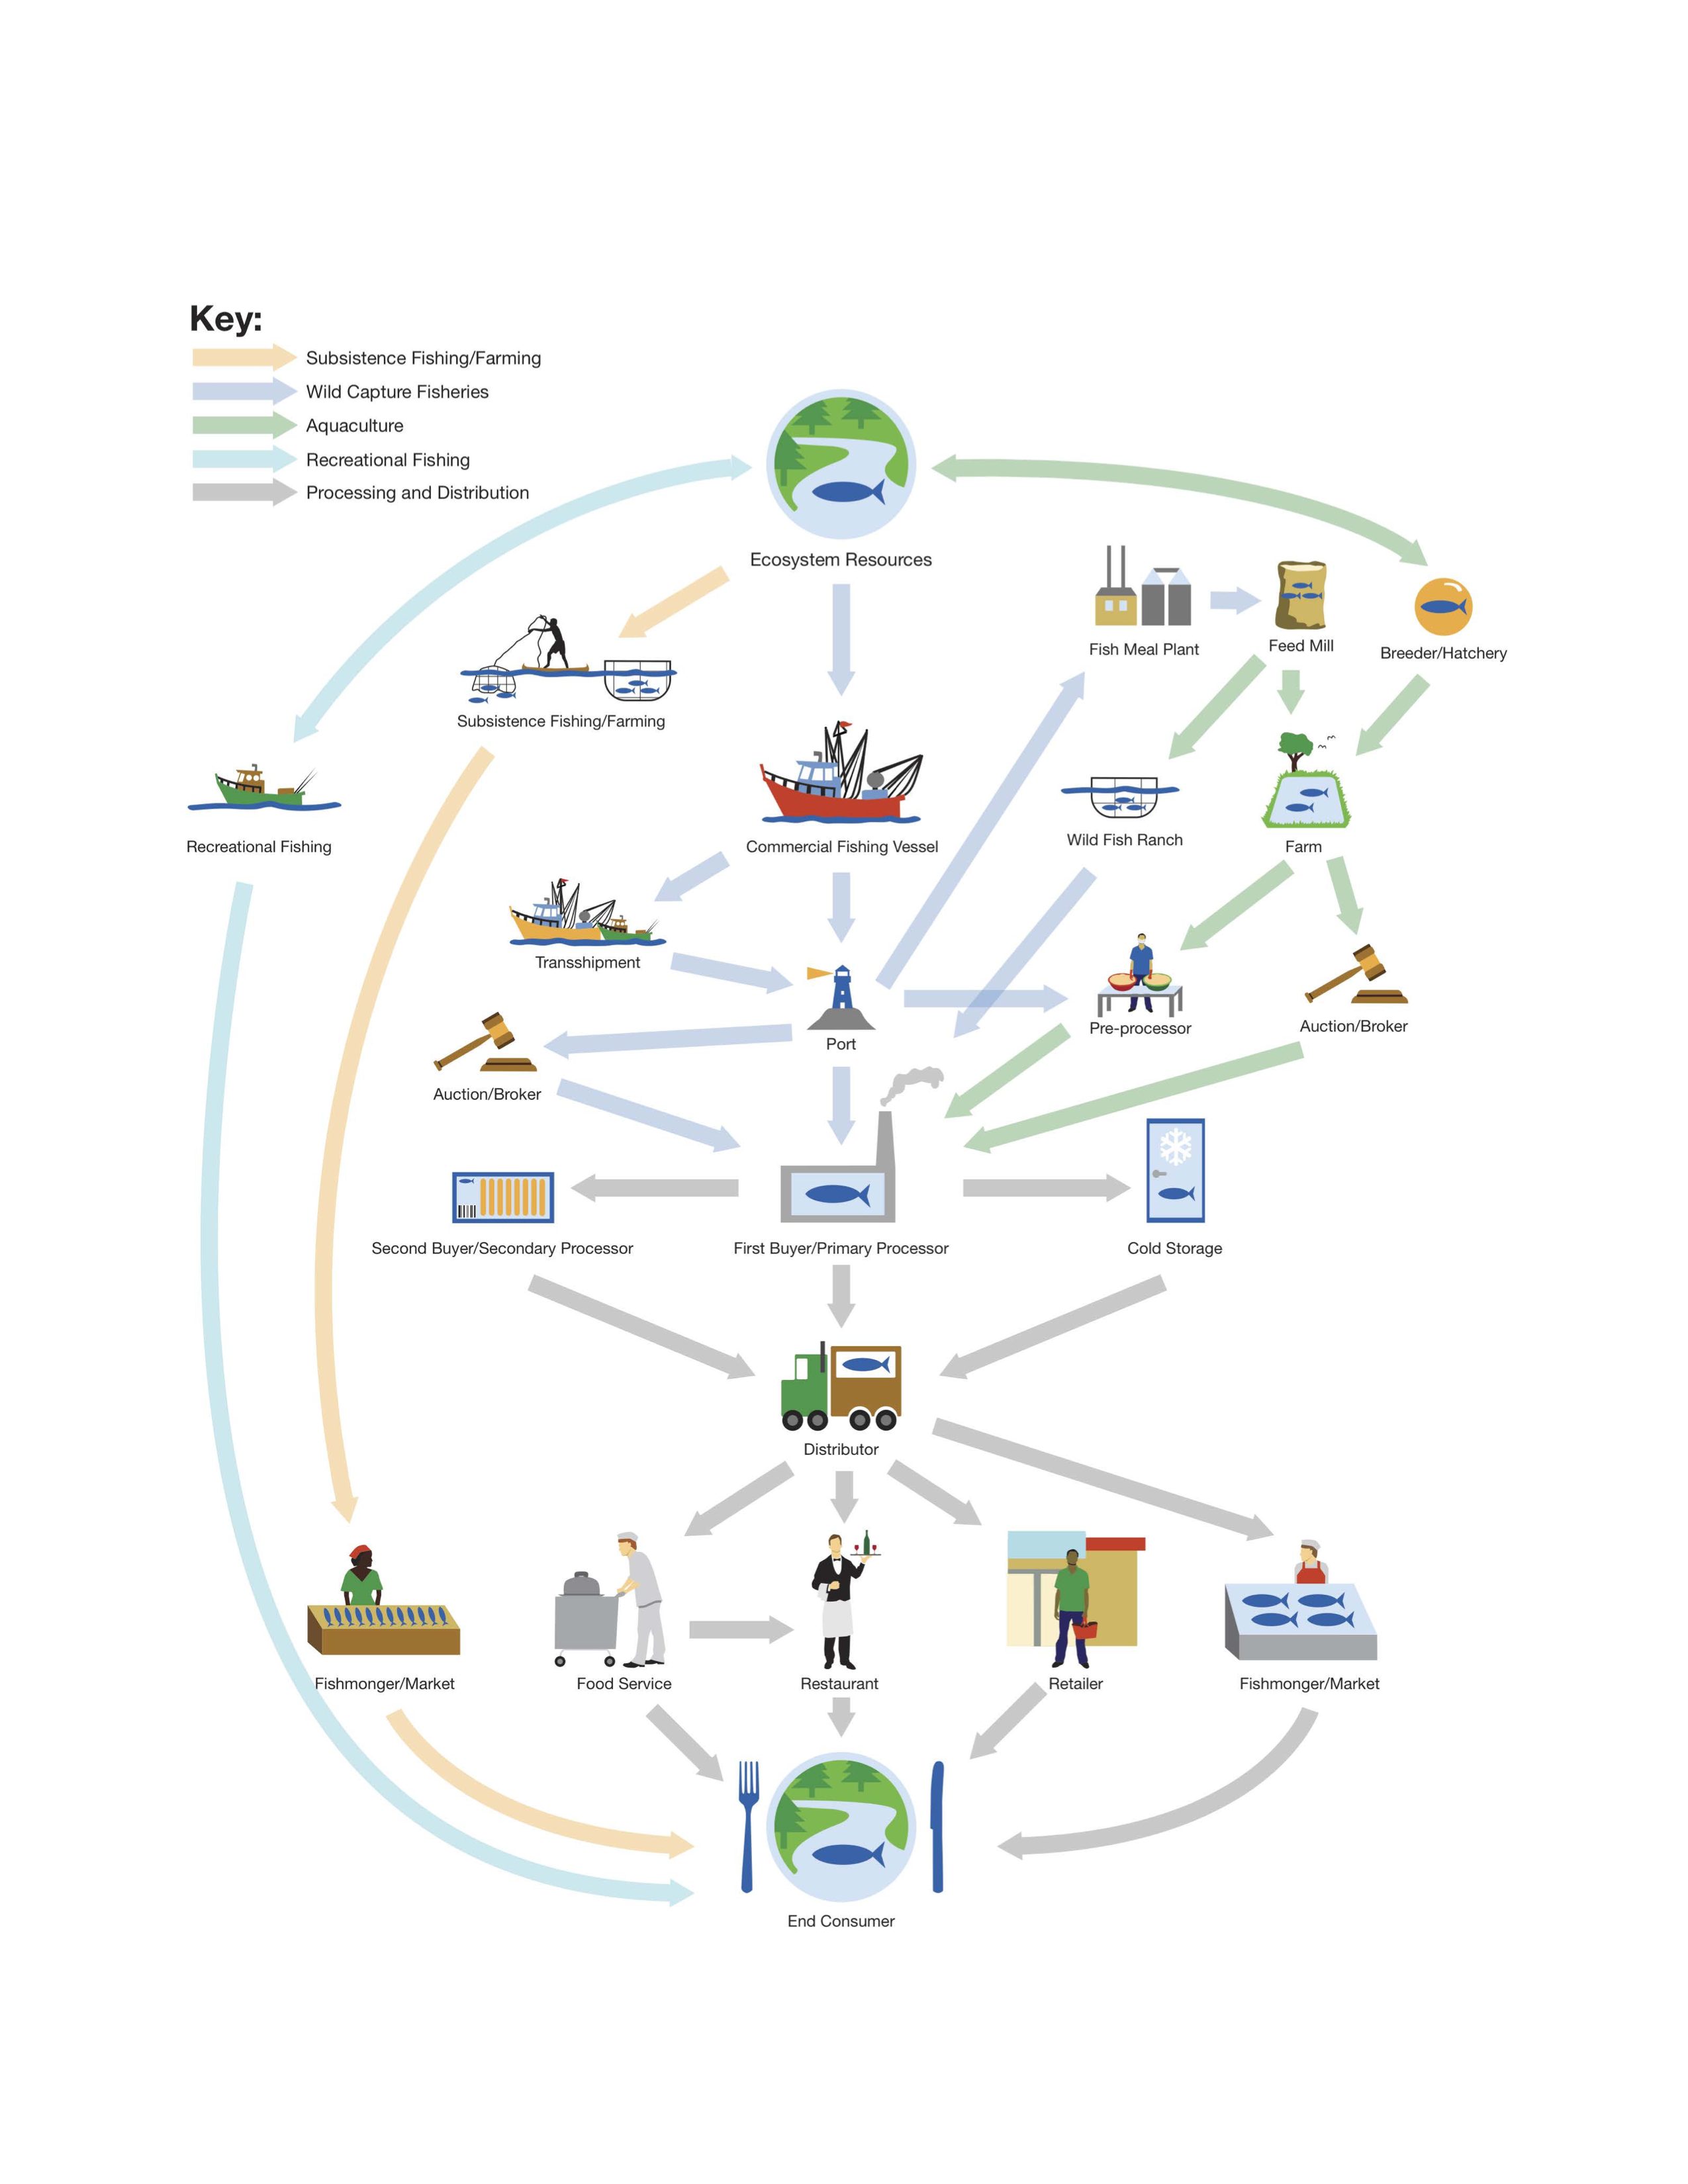
\includegraphics[height=22cm]{graphic_seafood_supply_chain.png}
\caption{\textbf{The Complexity of the Seafood Supply Chain}}
\emph{Source: Advancing Traceability in the Seafood Industry, FishWise}
\end{figure}
\newpage

\subsubsection{A seafood supply chain prototype}
A team at Intel is using \textbf{Hyperledger Sawtooth} to build a traceability prototype that combines the distributed ledger, IoT sensors, and advanced communications to track telemetry parameters throughout capture, processing, and transit. 

Sensors attached to the fish when it is caught record data such as location, temperature, and humidity. 
This data is recorded in the ledger, along with further events in the processing of the fish: ownership changes, transport company, storage temperature range, and so on. 
The ledger can also provide analytics for regulatory enforcement and scientific analysis of fish harvesting and consumption.

This prototype highlights the benefits of Hyperledger Sawtooth as a platform for tracing assets. 
The lightweight, highly decentralized consensus protocol in Sawtooth (proof of elapsed time) is particularly well-suited to a diverse, distributed ecosystem where thousands of validating nodes may be required. 
Broad participation in the ledger reflects the cross-industry nature of the seafood supply chain. 

\subsubsection{Asset tracking touches on different issues}
Asset tracking touches on several issues not generally seen in ledgers for financial products. 
For example, asset tracking requires handling diverse data types, such as the composite format required for telemetry and environmental sensing. 
Sawtooth accommodates both domain-specific data and the transaction families that operate on it, including data constraints such as verifying the calibration of a sensor.

Blockchain promises a number of benefits for cross-industry traceability. 
Most of all, these technologies can help establish a community of participants and an authoritative record of provenance. 
The blockchain's decentralized fault-tolerance enable updates from a wide range of nodes, including fishing boats, trucks, cold-storage facilities, retail stores, and restaurants. 

Beyond traceability, digitizing assets opens the door for completely new markets such as, for example, monetization of provenance.
